% This LaTeX document needs to be compiled with XeLaTeX.
\documentclass[10pt]{article}
\usepackage[utf8]{inputenc}
\usepackage{graphicx}
\usepackage[export]{adjustbox}
\graphicspath{ {./images/} }
\usepackage{amsmath}
\usepackage{amsfonts}
\usepackage{amssymb}
\usepackage[version=4]{mhchem}
\usepackage{stmaryrd}
\usepackage[fallback]{xeCJK}
\usepackage{polyglossia}
\usepackage{fontspec}
\setCJKmainfont{Noto Serif CJK JP}

\setmainlanguage{polish}
\setmainfont{CMU Serif}

\title{LIGA MATEMATYCZNA \\
 im. Zdzisława Matuskiego \\
 FINAモ \\
 25 kwietnia 2016 \\
 SZKOŁA PODSTAWOWA }

\author{}
\date{}


\begin{document}
\maketitle
ZADANIE 1.\\
Znajdź wszystkie liczby czterocyfrowe podzielne przez 4 o sumie cyfr równej 4.

\section*{ZADANIE 2.}
Duży prostokąt o obwodzie 136 cm podzielono na siedem przystających prostokątów tak, jak na rysunku. Oblicz pole dużego prostokąta.\\
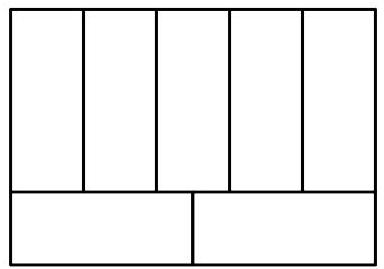
\includegraphics[max width=\textwidth, center]{2024_11_21_3b7d6c9f839d6cd4746cg-1}

\section*{ZADANIE 3.}
Wykaż, że liczba \(10^{45}+2\) jest podzielna przez 6.

\section*{ZADANIE 4.}
Tysiąc punktów umieszczono równomiernie na okręgu i ponumerowano kolejno od 1 do 1000. Jaki numer ma punkt leżacy naprzeciw punktu o numerze 657 ?

\section*{ZADANIE 5.}
Ramię trapezu równoramiennego ma długość 5 cm . Obwód trapezu jest równy 28 cm . Prosta przechodząca przez środki podstaw podzieliła ten trapez na dwie figury o obwodach po 18 cm . Oblicz pole trapezu.


\end{document}